\chapter{Notizen, Struktur}\label{ch:Notizen}

\begin{tcolorbox}[colback=yellow!10!white, colframe=red!75!black, title=\textbf{PROJEKT NOTIZEN}]
Hier werden zunächst nur grobe Notizen / Informationen gesammelt. Diese binden bereits BibTex Zitationen mit ein, sind aber nur grob sortiert.

\textbf{Hinweis:} Die Struktur dieses Kapitels spiegelt \textbf{nicht} die echte Struktur dieser Arbeit wieder. Es handelt sich hier nur um eine Sammlung von Themenkomplexen.
\end{tcolorbox}

Forschungsfragen des Masterprojektes:\todo[inline]{Forschungsfragen kommen in Ch.1, Erläuterung sollte folgen.}

\begin{description}
    \item[RQ1]\label{RQ1} Wie kann aus Userstories passender funktionaler Quellcode und zugehöriger Text erzeugt werden?
    \item[RQ2]\label{RQ2} Wie hoch ist der Automatisierungsgrad?
\end{description}

Zunächst die grobe Unterteilung in die einzelnen Themenbereiche, die für diese Arbeit betrachtet werden sollen. Hier werde ich zunächst Notizen zu bestimmten Papers/Arbeiten sammeln, damit ich die Citations bereits einfügen kann.

% ##################################### SUBSECTION #####################################

\subsection{Generelle Informationen}

Die Forschungsfragen \ref{RQ1} und \ref{RQ2} sollen in dieser Arbeit hinsichtlich des aktuellen Forschungsstandes beantwortet werden. Zur Sammlung von relevanten wissenschaftlichen Arbeiten lehne ich mich an \cite{kitchenhamGuidelinesPerformingSystematic2007} an, welches primär für Systematische Literatur Reviews geschrieben wurde.

Die Idee ist hier einen Prozess zu definieren, anhand relevante Arbeiten gesammelt und konzentriert werden. Die dabei wichtigesten \textasciitilde 20 Arbeiten werden gesammelt und analysiert. Damit soll in Kapitel \ref{ch:Verwandte Arbeiten} eine konkrete Analyse und Aufarbeitung dieser Arbeiten geschehen. Hier werden auch Arbeiten zu gleichen Themenbereichen gegenüber gestellt und verglichen.

Unabhängig von diesem Prozess habe ich selbständig relevante wissenschaftliche Arbeiten gesucht, welche in den Prozess mit eingebunden werden.

\subsubsection{Informationsbeschaffung wissenschaftlicher Literatur}

Wie bereits angeführt soll im Ramen dieser Arbeit eine Analyse vorhandener Literatur stattfinden. Dabei ergeben sich Thematische Schwerpunkte welche der direkten Beanwortung der Forschungsfragen dienen:

\begin{itemize}
    \item Generierung von Quellcode aus Anforderungen
    \item Automatisierungsgrad von LLM (Multi-Agent) Systemen \textit{(für Quellcode Generierung)}
\end{itemize}

Weiterhin gibt es verschiedene Themenkomplexe welche durch ihre unmittelbare Nähe zu den Forschungsfragen \textit{oberflächlich} analysiert werden sollen:

\begin{itemize}
    \item Quellcode Generation durch Multi-Agent Systeme
    \item Generation von User Stories
    \item Generation von Tests (Unit, E2E, Integration, UAT)
    \item Evaluation von Ergebnissen (LLM-Judges, etc.)
\end{itemize}

\subsubsection{Meta Analyse}

Hier soll zunächst die Outline für eine Meta Analyse definiert werden. Fokus der Analyse ist es, möglichst relevante wissenschaftliche Arbeiten zu sammeln und zu analysieren. Hinsichtlich des vorherigen Unter-Kapitels und in Betrachtung der Empfehlungen von \cite{kitchenhamGuidelinesPerformingSystematic2007} verfolge ich folgende Strategie:

\begin{enumerate}
    \item Definition von Inklusions/Exklusions-Kriterien
    \item Schlüsselwort Sammlung, daraus Queries definieren
    \item Sammlung durch akademische Tools (IEEExplore, arXiv, etc.)
    \item Bündelung und Sortierung von Ergebnissen
    \item Filtern der Ergebnisse
\end{enumerate}

Nach diesem Prozess sollten sich ca \textasciitilde 20 wissenschaftliche Arbeiten mit starker Relevanz ergeben.

\subsubsection{Umsetzung Meta Analyse}

\textbf{Strategie 1: SLR ähnliche Analyse via IEEExplore}

\begin{enumerate}
    \item Definition einer Query
    \item Anwendung Inclusion Criteria (IC)
    \item Anwendung Exclusion Criteria (EC)
    \item Screening (Manual?=)
\end{enumerate}

\textbf{Query}

Um möglichst viele Paper auf einmal zu gewinnen wird eine Query via IEEE Xplore ausgeführt. Hier wird bereits ein IC angewendet, da IEEE Xplore diese Funktionalität Diese sieht wie folgt aus:

\begin{verbatim}
    ("Large Language Model" OR LLM OR "Generative AI") 
    AND ("User Story" OR Requirement) 
    AND ("Code Generation" OR Autonomous OR "Multi-Agent")
\end{verbatim}
= 524 Arbeiten

\textbf{Inclusion Criteria / Inklusionskriterien}

\begin{enumerate}
    \item Publikation zwischen 2023 und 2026
    \item Arbeit behandelt die Transformation von natürlichsprachlich formulierten Anforderungen in Quellcode
    \item Arbeit nutzt LLMs / Agentic Frameworks / Multi-Agent-Systeme
    \item Arbeit evaluiert ihre Ergebnisse oder beschreibt die Architektur des Systems (am besten auch den Grad der Automatisierung)
\end{enumerate}

\begin{figure}
    \centering
    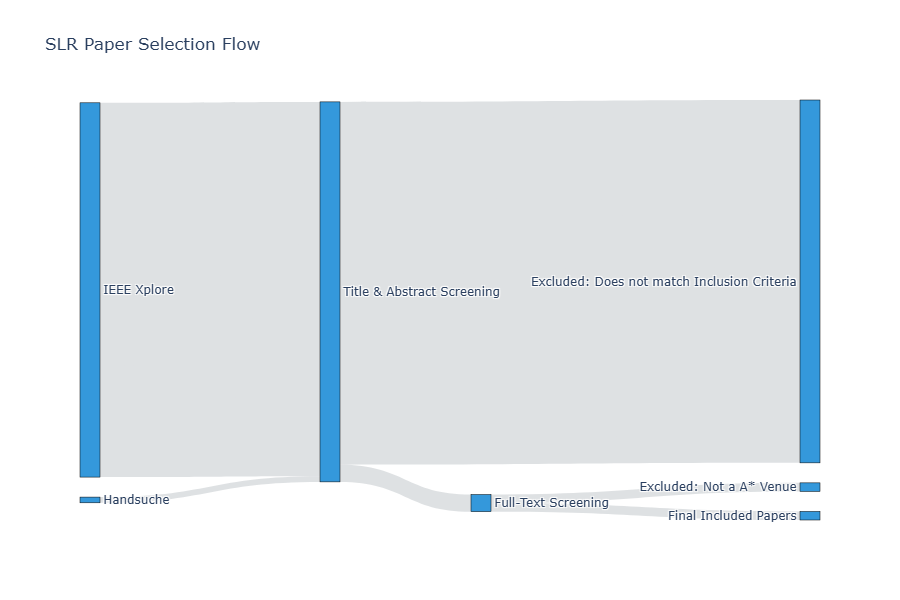
\includegraphics[width=1\linewidth]{images/selection_plot.png}
    \caption{Auswahl der Arbeiten}
    \label{fig:paper_selection}
\end{figure}

% \begin{enumerate}
%     \item Thematische Abarbeitung der Abstracts nach den IC:
%     \begin{enumerate}
%         \item Publikation zwischen 2023 und 2026
%         \item Arbeit behandelt die Transformation von natürlichsprachlich formulierten Anforderungen in Quellcode
%         \item Arbeit nutzt LLMs / Agentic Frameworks / Multi-Agent-Systeme
%         \item Arbeit evaluiert ihre Ergebnisse oder beschreibt die Architektur des Systems (am besten auch den Grad der Automatisierung)
%     \end{enumerate}
% \end{enumerate}

\textbf{Vorgehen}

\subsection{User Stories \& Requirements Engineering}

\subsubsection{User Acceptance Testing}

\cite{varpeUserAcceptanceTest2025} extrahiert aus Anforderungsdokumenten direkt User Acceptance Tests (UAT).\todo[inline]{Klären wie Acronyms zu behandeln sind! Glossary am Ende der Arbeit?} 
Die Idee selbst ist nicht neu, es wurde beispielsweise bereits aus UML-Diagrammen und XML Daten UAT generiert, dies erfordert allerdings einen weiteren Prozessschritt zur Aufbereitung der Anforderungen. Dieser Prozess lässt sich wie in \cite{varpeUserAcceptanceTest2025} gezeigt wird, auch mit einer LLM basierten Methodologie umsetzen, wobei echte Anforderungsdokumente aus \cite{ferrariPUREDatasetPublic2017a} als Testdaten dienen. Ein System aus 2 LLM-Agenten genügt hier für vielversprechende Ergebnisse.

\textbf{Aber:} Die Methodologie des Papers ist nicht unbedingt 100\% klar. Die Bewertung der Ergebnisse erfolgt via LLM-As-A-Judge und behauptet eine Coverage der Anforderungen von bis zu 72\%. Eine (heuristische?) Analyse via BERTScore wurde nur auf \textbf{1} Beispiel ausgeführt.

\textbf{Extra Note:} der Datensatz aus \cite{ferrariPUREDatasetPublic2017a} ist nicht uninteressant, da es hier eine große Menge and Anforderungen gibt die man evtl. für andere Zwecke nutzen kann. 

\subsection{Software Design}

\subsection{Code Generation}

\subsection{Automatisierung von Quellcode Generation}

\subsection{Evaluation von Resultaten}

Um die Ergebnisse von verschiedenen LLMs und Lösungsansätzen für NL2Code vergleichen zu können, bedarf es Benchmarks. In Benchmarks werden... 

\subsubsection{Herausfoderungen akurater Bewertung}



\subsubsection{Kontamination von Datensätzen}

Eine weitere gravierende Herausforderung für Benchmarks ist die Kontimination der Datensätze. Moderne LLMs werden auf massiven Datenmengen trainiert. Wenn ein Benchmark auf Open Source Projekten basiert, ist es praktisch unvermeidbar dass diese Projekte ebenfalls in die Testdaten mit eingehen. 

\todo[inline]{Kontamination ist nicht das richtige Wort, außerdem braucht es heir eine Primärquelle für das Problem selbst. --> Overfitting?}

% --------------------------------------------------------------------------------------------
% --------------------------------------------------------------------------------------------
% --------------------------------------------------------------------------------------------

\todo[inline]{Ab hier test Sektion für Formattierung, etc.}
